\documentclass[11pt,a4paper,landscape]{article}
\usepackage[margin=12mm,top=14mm,bottom=14mm,headheight=12pt]{geometry}
\usepackage{fontspec}
\setmainfont{DejaVu Sans}
\newfontfamily\latinfont{DejaVu Sans}
\newfontfamily\japanfont[AutoFakeBold=1.5]{Droid Sans Fallback}
\XeTeXlinebreaklocale "ja"
\XeTeXlinebreakskip=0pt plus 1pt
\newXeTeXintercharclass\japanese
\newcount\jpchar
\jpchar="3000 \loop\XeTeXcharclass\jpchar=\japanese\advance\jpchar by1 \ifnum\jpchar<"3100\repeat
\jpchar="3400 \loop\XeTeXcharclass\jpchar=\japanese\advance\jpchar by1 \ifnum\jpchar<"A000\repeat
\jpchar="FF00 \loop\XeTeXcharclass\jpchar=\japanese\advance\jpchar by1 \ifnum\jpchar<"FFF0\repeat
\XeTeXinterchartoks 0 \japanese={\japanfont}
\XeTeXinterchartoks \japanese 0={\latinfont}
\XeTeXinterchartoks 4095 \japanese={\japanfont}
\XeTeXinterchartoks 4095 0={\latinfont}
\XeTeXinterchartokenstate=1
\usepackage{amsmath,amssymb,graphicx,xcolor,array,booktabs,fancyhdr,tikz}
\usetikzlibrary{arrows.meta,positioning}
\usepackage[unicode,colorlinks=true,urlcolor=teal]{hyperref}
\hypersetup{pdftitle={EP8各binの高k* CFとtree解析の再現性},pdfauthor={STAR 2021 P24iy internal study}}
\definecolor{navy}{HTML}{18354B}\definecolor{teal}{HTML}{007F83}\definecolor{pale}{HTML}{EDF5F7}\definecolor{warm}{HTML}{FFF1E4}
\color{navy}\pagestyle{fancy}\fancyhf{}
\fancyhead[L]{\scriptsize Au+Au fixed target / 2021 P24iy / $\Lambda$--$^4$He}
\fancyhead[R]{\scriptsize 完了済みEP8と入出力再現性 / 2026-11-20}
\fancyfoot[L]{\scriptsize raw signal・背景差引き前。CF規格化は $0.4\le k^*<0.5$ GeV/$c$。}
\fancyfoot[R]{\scriptsize\thepage}\renewcommand{\headrulewidth}{.3pt}
\setlength{\parindent}{0pt}\setlength{\parskip}{4pt}\setlength{\emergencystretch}{2em}\renewcommand{\arraystretch}{1.22}\raggedright
\newcolumntype{P}[1]{>{\raggedright\arraybackslash}p{#1}}
\newcommand{\ttl}[2]{{\small\color{teal}#1}\par{\fontsize{20}{25}\selectfont\bfseries #2}\par\vspace{2mm}}
\newcommand{\note}[1]{\par\colorbox{pale}{\parbox{\dimexpr\linewidth-5mm\relax}{\vspace{1mm}\small #1\vspace{1mm}}}\par}
\newcommand{\warn}[1]{\par\colorbox{warm}{\parbox{\dimexpr\linewidth-5mm\relax}{\vspace{1mm}\small #1\vspace{1mm}}}\par}
\newcommand{\figpage}[4]{\clearpage\ttl{#1}{#2}\begin{center}\includegraphics[width=\linewidth,height=.76\textheight,keepaspectratio]{#3}\end{center}{\small #4}\par}
\graphicspath{{/gpfs/mnt/gpfs01/star/pwg/yichikawa/git_STAR_3/star-analyzer/share/figure/20261120_lambda_ep8_cf_closure_report/}}
\begin{document}
\ttl{01 / 結論と確認範囲}{EP8の各binでも、高い $k^*$ の形状差が残る}
\textbf{完了済みの第二段階EP8出力から、各角度binを個別に規格化して比較した。}

\begin{minipage}[t]{.56\linewidth}\vspace{0pt}
\note{\textbf{高$k^*$の観察：0--60\%}\par
$0.8\le k^*<1.0$ GeV/$c$の窓積分から求めたCFは、8binすべてで\textbf{約0.899--0.923}。\par
各binに分けても、表示範囲の上側で1を下回る傾向が残る。}
\par
\vspace{1mm}\begin{tabular}{lll}
\toprule $k^*$窓 [GeV/$c$] & EP合算 & 8binの範囲\\\midrule
0.5--0.6 & 0.9853 & 0.9659--1.0043 \\
0.6--0.8 & 0.9513 & 0.9383--0.9664 \\
0.8--1.0 & 0.9122 & 0.8990--0.9234 \\
0.6--1.0 & 0.9302 & 0.9171--0.9421 \\
\bottomrule\end{tabular}
\par

\vspace{2mm}
\textbf{読み取り方}\par
規格化域ではSEとMEの積分が一致するように揃える。その外側の高$k^*$で、同じ高さ・形に近づくかを確認する。ここでは0.5--1.0 GeV/$c$を調べる。
\end{minipage}\hfill
\begin{minipage}[t]{.41\linewidth}\vspace{0pt}
\note{\textbf{tree導入の再現性：同一条件の試験}\par
同じ10,000入力eventを使い、直接PicoDst解析とtree再読のQA108本＋pair1186本が完全一致した。非空pairヒスト587本を含む。}
\textbf{二つの問いを別に評価する}\par
1. 保存・再読で情報が変わるか\par
\quad 同一入力・同じME条件の再現性試験で確認。\par
2. 高$k^*$のCFが1へ近づくか\par
\quad 全統計EP8の各binで評価。\par
\vspace{2mm}
進行中のEP1/16/32・原点cut比較は、本資料の数値には含めていない。
\end{minipage}
\warn{数値は規格化後の窓積分比による形状の比較。event/ME共有・規格化の共分散を含む有意差検定や、$k^*\to\infty$の漸近値の推定は行っていない。}

\clearpage\ttl{02 / データと定義}{同じSE・MEに、同じ規格化を適用する}
\begin{minipage}[t]{.64\linewidth}\vspace{0pt}
\begin{tabular}{P{38mm}P{127mm}}
\toprule 対象 & 条件\\\midrule
データ & 2021 P24iy、較正対象388run。完了済み第二段階20期間。\\
保存・EP判定 & 保存/処理1,819,447,887。EP-valid 1,736,875,306、invalid 82,572,581。pairにはvalidを使用。\\
pool & 同じcent9 $\times$ Vz 10bin $\times$ EP 8bin。深度100、両方向bufferAll。\\
期間内の継続 & 同じ期間の元producer境界を越えてmixを継続する。\\
pairの選択 & $\Lambda$--物理$^4$Heのsignal。原点pair cutなし。\\
表示 & native幅0.005、4bin合成で0.02 GeV/$c$。上限1 GeV/$c$。\\\bottomrule
\end{tabular}
\[
\alpha_i=\frac{SE_i(H)}{ME_i(H)},\qquad C_i(k^*)=\frac{SE_i(k^*)}{\alpha_i ME_i(k^*)},\quad H=[0.4,0.5)
\]
\[
R_i(W)=\frac{SE_i(W)}{\alpha_i ME_i(W)}\qquad\text{（表・heatmapの高$k^*$窓積分比）}
\]
各EP binで$\alpha_i$を求める。centralityやEPを合成する場合はraw SE/MEを先に加算し、最後に一度規格化する。CFの単純平均は使わない。 軸外のunderflow/overflowは保存総数に含み、規格化・窓積分には混入させない。
\end{minipage}\hfill
\begin{minipage}[t]{.32\linewidth}\vspace{0pt}
\begin{center}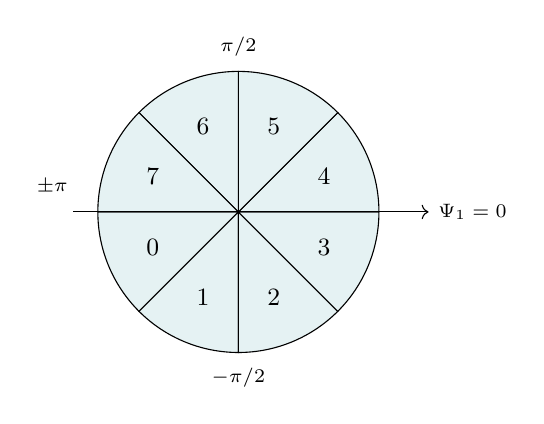
\begin{tikzpicture}[scale=1.05]
\foreach \i in {0,...,7}{\pgfmathsetmacro{\a}{-180+45*\i}\pgfmathsetmacro{\b}{\a+45}\pgfmathsetmacro{\m}{\a+22.5}\draw[fill=teal!10] (0,0)--(\a:1.7) arc (\a:\b:1.7)--cycle;\node[font=\small] at (\m:1.12){\i};}
\draw[->](-2,0)--(2.3,0)node[right,font=\scriptsize]{$\Psi_1=0$};
\node[font=\scriptsize] at (0,2){$\pi/2$};\node[font=\scriptsize] at (0,-2){$-\pi/2$};\node[font=\scriptsize] at (-2.25,.3){$\pm\pi$};
\end{tikzpicture}\end{center}
\small binは補正済み$\Psi_1$の角度区間を指す。保存indexは0--7、公称幅45度。境界の実判定は元コードのFloat\_t計算に従う。
\note{error barは$\alpha_i$固定でのhistogram誤差伝播。規格化の共分散・同eventからのpair相関は含めない。}
\end{minipage}

\figpage{03 / 0--60\%・全表示域}{EP8各binのCF：同じ軸で比較}{ep8_cf_c00_60_panels.pdf}{各binを個別に規格化。参照線$C=1$と比較する。EP合算の参照はraw SE/MEを合成してから規格化した値。背景差引き・purity補正前。}
\figpage{04 / 0--60\%・高$k^*$拡大}{8binとも、0.8--1.0 GeV/$c$で1を下回る}{ep8_cf_c00_60_highk_panels.pdf}{窓積分比は0.899--0.923。0.5--0.6 GeV/$c$のほぼ1から、高$k^*$側へ低下が続く。元histogram上限が1 GeV/$c$のため、それより上の収束はこの出力から評価しない。}
\figpage{05 / 割り算前の形状}{EP8各binのSEとME：規格化域でスケール}{ep8_seme_c00_60_panels.pdf}{表示はSE/SE$(H)$とME/ME$(H)$。同じ規格化域の積分を1へ揃えた形状比較であり、絶対pair数の同一性を意味しない。高$k^*$でSEが相対的に低くなる部分がCFの低下に対応する。}
\figpage{06 / 0--60\%・数値での比較}{高$k^*$窓の積分比をEP binごとに確認する}{ep8_highk_c00_60_table.pdf}{$R_i(W)=SE_i(W)/[\alpha_i ME_i(W)]$を使用。CF点の単純平均とは区別する。各binで規格化係数を個別に算出。同じbin内の複数窓は規格化を共有する。}
\figpage{07 / centrality別・主窓0.6--1.0 GeV/$c$}{centralityをそろえて、EP binの違いを見る}{ep8_highk_primary_heatmap_v2.pdf}{数値は各centrality・各EP binで独立に規格化した窓積分比。色の差は記述的な形状差で、共分散を含む有意差ではない。0--60\%の合成と独立cent9の結果を区別する。}
\figpage{08 / centrality別CF}{各centralityで8binを重ねる}{ep8_cf_six_centralities_overlay.pdf}{0--10、10--20、20--30、30--40、40--50、50--60\%の各条件。中心事象0--5、5--10、10--20\%でも全EP binで0.8--1.0の窓積分比が1未満（付録も参照）。周辺事象は統計と規格化の揺らぎが大きく、同じ強さで判断しない。}
\figpage{09 / 同じ入力・同じME条件でのclosure}{旧直接解析とtree再読：SE・MEが重なる}{closure_matched_seme.pdf}{run22159051の同じPicoDst先頭10,000 eventを入力。旧新とも$^4$He signal SE13、ME403（flow込み）。下段は新$-$旧のbin差。データ点は同一eventから作られたもので、独立標本としての統計比較ではない。}

\clearpage\ttl{10 / tree導入で何を確認できたか}{再現性の確認と、ME条件変更の評価範囲}
\begin{minipage}[t]{.56\linewidth}\vspace{0pt}
\begin{tabular}{P{50mm}P{94mm}}
\toprule 同一条件の実ROOT監査 & 結果\\\midrule
入力・再構成 & 同PicoDstの10,000入力、9,761再構成。\\
EP母集団 & seen9,761 / valid9,374 / rejected387。\\
元のME条件 & 深度20、cent9$\times$Vz10$\times$EP8、bufferAll、両方向、segment境界reset。\\
比較範囲 & 初段QA108＋pair1186。非空pair587を含む。\\
比較した項目 & 46,336,786セル（flow含む）。内容・誤差・Entries・軸・raw Sumw2の差ゼロ。\\
$^4$He signal & 旧新ともSE13 / ME403。規格化域はSE1 / ME24。\\
保存範囲 & compactは非選択prePID control540ヒストを再計算対象外とする。\\\bottomrule
\end{tabular}
\note{このsampleは入出力の再現性試験。signal SE13のため、高$k^*$の物理的な収束判定には使わない。}
\end{minipage}\hfill
\begin{minipage}[t]{.40\linewidth}\vspace{0pt}
\begin{center}\resizebox{.95\linewidth}{!}{\begin{tikzpicture}[>=Stealth,box/.style={draw=teal,fill=pale,rounded corners,text width=34mm,align=center,minimum height=10mm,font=\small},node distance=5mm and 6mm]
\node[box](p){同じPicoDst};\node[box,below left=of p](a){旧直接解析};\node[box,below right=of p](b){新producer};\node[box,below=of b](t){compact tree};\node[box,below=of t](v){replay};\node[box,below=of v](q){raw SE/ME};\node[box](o) at (a|-q){raw SE/ME};
\draw[->](p)--(a);\draw[->](p)--(b);\draw[->](b)--(t);\draw[->](t)--(v);\draw[->](a)--(o);\draw[->](v)--(q);\draw[<->,thick](o)--node[above,font=\small]{一致}(q);
\end{tikzpicture}}\end{center}
\textbf{全統計の条件は別に記録する}\par
本資料のEP8全統計は深度100・期間内継続。旧直接解析本番とmixing条件・収録範囲をそろえた全統計closureではない。\par
現在のEP8各binで残る高$k^*$の低下は、EP1/16/32・原点cut有無の進行中比較と合わせて評価する。
\end{minipage}
\warn{同一条件の試験で保存・再読の結果が再現されることを確認した。CF形状差の原因を、tree形式・EP幅・統計・pool設定のどれかに直ちに帰属させることは避ける。未較正81runと初段未回収34件は保留のまま。}

\figpage{付録 / 独立cent9}{0--5\%と5--10\%も別に確認する}{ep8_cf_nine_cent9_overlay.pdf}{cent9=0--8を個別に規格化したCF。0--60\%の合成はcent9=2--8。周辺centralityやplaneの規格化域が空の場合は、未評価と表示してゼロ値を作らない。 周辺の極低統計binは形状判断の対象外とする。 60--70\%、70--80\%では規格化域のSEが1または0のbinがあり、大きく揺らぐ。}
\clearpage\ttl{再現情報}{使用ファイルと、今回の作業範囲}
\small
\begin{tabular}{P{48mm}P{210mm}}
\toprule 項目 & 保存先・定義\\\midrule
全統計EP8 SUMS ID & \texttt{2D07F680577123CABC16FDD9159CFD9E}\\
完了済み入力 & \path{rootfile/femto_lambda_period_mix100_20261119_001/output_roots_20261120.list} （20 ROOT）\\
EP8 raw集約・元証跡 & \path{rootfile/femto_lambda_ep_merging_systematics_20261120_001/cf_baseline_ep8Off_002/}\\
今回の数値・独立検証 & \path{rootfile/lambda_ep8_cf_closure_report_20261120_001/}\\
旧新closure実ROOT & \path{rootfile/femto_lambda_tree_implementation_20261117_001/} の\texttt{baseline\_10k.root}, \texttt{producer\_compact\_10k.root}, \texttt{compact\_replay\_10k.root}\\
closure監査 & 今回作業dirの\texttt{closure\_root\_audit.json}。保存histogramの独立再読、event tree payload未読。\\
元の解析条件 & \path{config/mainconf/main_auau3p85_anaFemtoLambda_4He_tree_periodMix100.yaml}。本番snapshotは対応runmeta/configlogで保管。\\
資料・再生成 & \path{share/figure/20261120_lambda_ep8_cf_closure_report/}\\\bottomrule
\end{tabular}
\note{本資料作成では、既存histogramの射影・加算・規格化・作図を行う。新しいmixingやPicoDst再処理、job投入、元ROOT/進行中job/解析source/configの変更は行わない。}
\vspace{3mm}
独立計算は12,113 checksを通過。各cent9でのEP全binの和（軸外binを含む）、各planeの規格化域の積分比1、元のCF・高$k^*$窓の再現を確認した。元集約JSONのSHA256は読取前後で不変。\par
source metadataと元ROOTの選択・run/EP較正条件を確認し、matched sampleの直接解析とtree再読を比較した。source revisionは\texttt{unrecorded}のため、再現には保存されたsource/config/dependency指紋と入力順序も使用する。

\end{document}
